\chapter{Hidden Markov Map Matching}

Source: \cite{newson2009hidden}.

\section{论文动机}

\subsection{原始数据}

the raw input
data consists of vehicle \term{locations} measured by GPS, Each measured point consists of a time-stamped
latitude/longitude pair. 

The \term{roads} are also represented in the
conventional way, as a graph of nodes and edges.
The \term{nodes} are at
intersections, dead ends, and road name changes, and the edges
represent road segments between the nodes. Some \term{edges} are
directional to indicate one-way roads. Each node has an associated
latitude/longitude to indicate its location, and each edge has a
polyline (折线) of latitude/longitude pairs to represent its geometry.

\section{其他论文的方法}

平滑曲线匹配:create a (possibly smoothed) curve
from the location measurements and attempt to find matching
roads with similar geometry

\begin{example}
White et al. 
present four algorithms, starting with the simple, nearest match
scheme. 
Their second algorithm \textbf{adds orientation information to
the nearest match approach}, comparing the measured heading to
the angle of the road. Their third algorithm evolves the second
algorithm to \textbf{include connectivity constraints}, and their fourth
algorithm does \textbf{curve matching}. 

\begin{remark}
    their most sophisticated algorithm, the fourth one, was
outperformed by the simpler second algorithm.
\end{remark}
\end{example}

通过拓扑结构建模:builds up a
topologically feasible path through the road network. Matches are
determined by a similarity measure that weights errors based on
distance and orientation. The algorithm was found to perform flawlessly, even though the GPS data was collected while
\term{Selective Availability} was turned on, leading to noisier location
measurements than are available now.

模糊匹配策略:Kim and Kim look at a
way to measure \textbf{how much each GPS point belongs to any given road}, taking into account its distance from the road, the shape of
the road segment, and the continuity of the path. The measure is
used in a \textbf{fuzzy matching scheme} with learned parameters to
optimize performance.

Brakatsoulas et al. Their
algorithm uses variations of the \term{Fréchet distance} to match the
curve of the GPS trace to candidate paths in the road network.

\begin{remark}
    One potential problem with purely geometric approaches is \textbf{their
sensitivity to measurement noise and sampling rate.} 
Connecting the dots of a set of noisy measurements sampled at a
slow rate would not match well with the road geometry, especially
\textbf{direction information}.
\end{remark}

基准方法:将GPS点匹配到最近邻的路上

\begin{remark}
    result in extremely unreasonable paths involving strange U-turns, inefficient looping, and overall bizarre driving
behavior.
\end{remark}

\section{论文贡献}

\begin{itemize}
    \item maintaining a principled approach to the problem while simultaneously making the algorithm robust to location data that is both \textbf{geometrically noisy and temporally sparse}
    \item a test of our map matching algorithm where we vary the levels of noise and sparseness of the sensed location data over a 50 mile urban drive
\end{itemize}

\section{论文模型-Hidden Markov Model}

The HMM models processes that involve a path through many
possible states, where some state transitions are more likely than
others and where the state measurements are uncertain.

\subsection{HMM}

\begin{figure}[h]
    \centering
    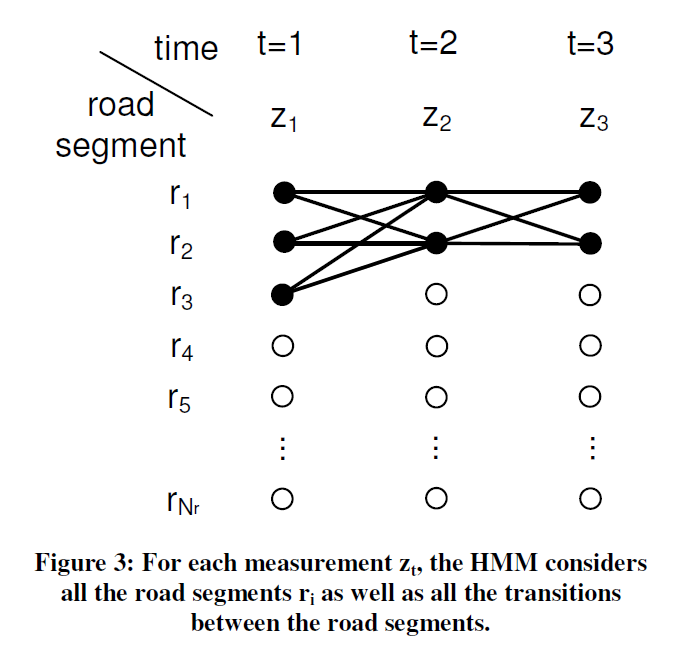
\includegraphics[scale=0.4  ]{hmm-hmm-of-observation.png}
\end{figure}

\begin{itemize}
    \item HMM状态:$ N_{r} $ individual  road  segments $ r_{i},  i=1 \ldots N_{r} $
    \item 状态的测量:每次带噪声的位置数据 $ Z_{t} $
    \item 候选路径:有很多,可能有很曲折的
    \item 目标:将每个GPS点匹配到合适的路段上
\end{itemize}

\subsection{已知在这个路段得到这个GPS点位置的概率估计}

\begin{figure}[h]
    \centering
    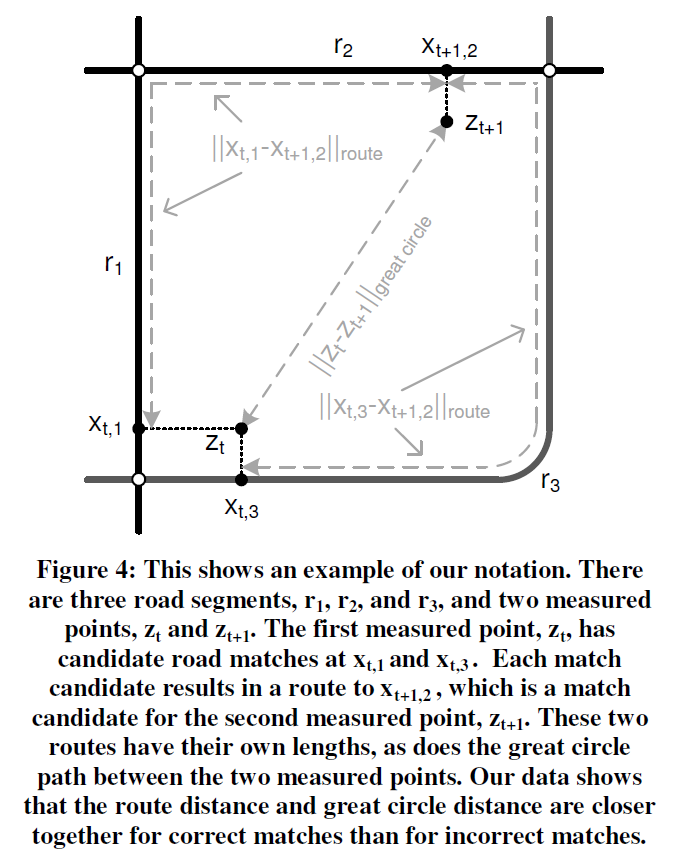
\includegraphics[scale=0.4  ]{HMM-mapping.png}
\end{figure}

对于给定的$z_{t},r_{i} $有\term{emission probability}$ x_{t, i}$

估计方法:
The \term{great circle distance} on the surface of the earth between the measured point and the candidate match is $ \| z_{t}- x_{t, i} \|_{great\_circle}$. For the correct match, this difference is due to GPS noise. model GPS noise as zero-mean Gaussian 


